\documentclass[sn-apa]{sn-jnl}% APA Reference Style 

\usepackage{graphicx}%
\usepackage{multirow}%
\usepackage{amsmath,amssymb,amsfonts}%
\usepackage{amsthm}%
\usepackage{float}%
\restylefloat{table}
\usepackage{makecell}%
\usepackage{mathrsfs}%
\usepackage[title]{appendix}%
\usepackage{xcolor}%
\usepackage{textcomp}%
\usepackage{manyfoot}%
\usepackage{booktabs}%
\usepackage{algorithm}%
\usepackage{algorithmicx}%
\usepackage{algpseudocode}%
\usepackage{listings}%

\raggedbottom

\begin{document}

\title[Article Title]{Time Series Forecasting Using Recurrent Neural Networks Based on Recurrent Sigmoid Piecewise Linear Neurons}


\author[1]{\fnm{Victor} \sur{Sineglazov}}\email{svm@nau.edu.ua}
\equalcont{These authors contributed equally to this work.}

\author*[1]{\fnm{Vladyslav} \sur{Horbatiuk}}\email{vladyslav.horbatiuk@npp.nau.edu.ua}

\affil*[1]{\orgdiv{Department of Aviation Computer Integrated Complexes}, \orgname{National Aviation University},
\orgaddress{\street{Liubomyra Huzara Ave 1}, \city{Kyiv}, \postcode{03058}, \country{Ukraine}}}


\abstract{We propose a new recurrent sigmoid piecewise linear neuron that can be used in neural networks to model time series when solving forecasting problems. The neuron is simpler than widely used long short-term memory and gated recurrent unit neurons and can be used as a drop-in replacement of these neurons. Simpler model of the new neuron results in faster training and inference of networks composed of such neurons. Besides theoretical analysis of the neuron's mathematical model the experiments on real world time series were performed to measure and compare accuracy of networks with different structures and used neuron types. Results of experiments show that networks with the new neuron achieve similar or slightly better accuracy while having noticeably faster training and inference time.}

\keywords{recurrent neural networks, time series forecasting, sigmoid piecewise linear neuron, long short term memory neuron, gated recurrent unit neuron}

\maketitle

\section{Introduction}\label{sec1}

Forecasting is the process of predicting future events based on past and present data. Time series forecasting is a type of forecasting that predicts future events based on time-stamped data points. Time series forecasting models are an essential tool for any organization or individual who wants to make informed decisions based on future events or trends. From stock market forecasts to weather forecasts, time series models help us understand and predict changes over time. Forecasting is a part of statistical modeling that is widely used in various problems solutions and it is an important element of decision-making activity because whether an effective decision is made depends on forecasts accuracy. Performing short-term and/or long-term and reliable time series forecasting remains as relevant as ever across a vast number of application domains, including healthcare \citep{kaushik2020ai}, meteorology \citep{faisal2022neural}, physiology \citep{ghassemi2015multivariate}, energy systems \citep{amasyali2018review}, econometrics \citep{sineglazov2018forecasting} amongst many others. 

Nowadays artificial neural networks are the most popular and widely used tool for many problems in areas like computer vision, natural language processing, autonomous driving and more. In the time series forecasting domain recurrent neural networks (RNNs) are often employed \citep{hewamalage2021recurrent} due to their suitability for sequential data processing and modeling. The popular choices for recurrent neurons to be used in RNNs are long short-term memory (LSTM) neuron \citep{hochreiter1997long} and gated recurrent unit (GRU) neuron \citep{cho2014learning} since these neurons are designed to better capture long-term dependencies in sequential data.

RNNs composed of multiple layers of LSTM or GRU neurons are able to model pretty complex recurrent functions which is good when the time series in question has a lot of available data points, but can be a disadvantage for smaller time series leading to overfitting and increased variance of predictions. Another practical drawback is relatively high training and inference speed of the model. In the paper we suggest a new recurrent sigmoid piecewise linear (RSPL) neuron which is based on sigmoid piecewise linear (SPL) neuron \citep{zgurovsky2018structural} and can be viewed as a simplified version of LSTM and GRU neurons (or just a GRU neuron, since it can also be considered a simplified version of LSTM neuron). As a result of RSPL neuron having a simpler model the networks composed of layers of this neuron are faster during both training and inference stages. Besides that, experiments on real time data have shown that replacing LSTM/GRU neurons in networks with RSPL neuron does not lead to decrease in accuracy on small time series.

The paper is organized as follows. An overview of related works is given in Sect. \ref{sec2}. Sect. \ref{sec3} gives a formal time series forecasting problem statement that is explored in this paper. Sect. \ref{sec4} presents a short overview of LSTM and GRU neurons. Sect. \ref{sec5} starts with an overview of SPL neuron and proceeds with introduction of RSPL neuron. Results of practical experiments on real world time series are given in Sect. \ref{sec6}.

The main contributions of this paper can be summarized as follows. This paper:
\begin{enumerate}
\item Proposes a new recurrent neuron - RSPL neuron - that may be used in layers of recurrent networks to model time series.
\item Explores the connection between RSPL, LSTM and GRU neurons.
\item Conducts practical experiments on real world time series to compare accuracy, training and inference speed of networks composed of layers of LSTM, GRU and RSPL neurons.  
\end{enumerate}

\section{Related works}\label{sec2}

There are many different types of time series forecasting models, each with their own strengths and weaknesses:

\begin{itemize}
\item ARIMA based models \citep{box2015time}.
\item Regression trees based models \citep{breiman2017classification}, including boosting trees approaches \citep{chen2016xgboost}.
\item Artificial intelligence models, notably approaches based on artificial neural networks (ANNs) \citep{tealab2018time}, \citep{sineglazov2014using}, \citep{sineglazov2013algorithm}.
\item Hybrid approaches, e.g. in \citep{fawzy2022comparative} authors use a combination of ANNs and ARIMA models, in \citep{ngo2022developing} a combination of ARIMA and support vector regression \citep{awad2015support} is trained using firefly-inspired optimization algorithm \citep{fister2013comprehensive}, \citep{sineglazov2018forecasting} uses ANN and GMDH-based \citep{ivakhnenko1995review} algorithm for simultaneous optimization of network structure and parameters.
\end{itemize}

ANNs are becoming increasingly popular in time series forecasting due to their ability to model complex, non-linear relationships within data. Traditional statistical methods often assume linearity and may struggle with intricate patterns and interactions in real-world time series data. ANNs, however, can automatically learn these patterns without explicit programming, making them highly adaptable to diverse applications. Additionally, advances in computing power and the availability of large datasets have made it feasible to train deep learning models efficiently. The flexibility of neural networks to incorporate various types of data, such as exogenous variables and high-frequency data, further enhances their predictive accuracy. This combination of adaptability, improved computational resources, and superior performance in capturing non-linear dependencies is driving the growing adoption of ANNs in time series forecasting.

Specific kind of ANNs - recurrent neural networks - are particularly well suited to time series forecasting due to their inherent ability to retain and utilize sequential information. Unlike traditional neural networks, RNNs have loops in the "data flow" that allow information to persist, effectively creating a form of memory. This enables RNNs to maintain context and learn temporal dependencies within the data, which is crucial for accurately predicting future values based on historical trends. Their architecture is specifically designed to handle time-dependent data, making them well-suited for capturing the dynamic behavior and evolving patterns in time series. Moreover, popular recurrent neurons like LSTM and GRU address the limitations of standard RNNs, such as the vanishing gradient problem, by better managing long-range dependencies and improving the stability of the learning process. This makes RNNs highly effective for a wide range of time series forecasting tasks, from financial market analysis to weather prediction.

\section{Time series forecasting problem}\label{sec3}
There are two different classes of time series: stationary and non-stationary:

\begin{itemize}
\item Stationary time-series data is one where the statistical properties of the data do not change over time. In other words, the data does not exhibit any trend, seasonality, or other patterns that would cause these statistical properties to change. The random error is the only source of variability in the data set.
\item Non-stationary time-series data is a time-series data set that exhibits a trend or a seasonal effect. The random error is no longer the only source of variability in the data set. Non-stationary time-series data requires additional pre-processing, such as detrending or differencing, to remove the non-stationary before modeling and forecasting can be done accurately. 
\end{itemize}

Time series forecasting problem considered in this paper can be stated as follows.

\textbf{Given}: a time series ${x_1, ..., x_N}$, generated by some probabilistic process $ \{X_t\} $ with unknown joint distributions $p(x_{t+k}, x_{t}, x_{t-1}, ..., x_{t-n})$. The process $ \{X_t\} $ can be either stationary or non-stationary. If the process is non-stationary, in the general case this forecasting problem has no solution, since the probability distributions of a non-stationary series in theory can change "at will", and distributions in the future may have nothing in common with the distributions on the basis of which the existing time series was generated. However, in practice, changes in the probability distributions of non-stationary processes over time do not occur completely randomly. Therefore, predictive models tuned to the available time series data usually perform satisfactorily over a certain period of time, even if the corresponding process is non-stationary. 

\textbf{Find}: a predictive model of the form $ \hat{x}_{t+k} = f^*(x_{t}, ..., x_{t-n}) $ that minimizes the mathematical expectation of the error:
\begin{equation}
f^* = argmin_f
	\{ E_{p(x_{t+k}, x_{t}, x_{t-1}, ..., x_{t-n})} [ L(f(x_{t}, ..., x_{t-n}), x_{t+k}) ] \},\label{eq1}
\end{equation}
where:

\begin{itemize}
\item $L: \mathbb{R} \times \mathbb{R} \to \mathbb{R}_{\geq 0} $ - is the error function; common choices are quadratic $ L(x, \hat{x}) = (x-\hat{x})^2 $ or absolute error $ L(x, \hat{x}) = |x-\hat{x}| $ functions;
\item $k$ - forecasting horizon, i.e. how many steps ahead the forecast should be performed.
\end{itemize}

Since it is generally impossible to calculate the real mathematical expectation (the corresponding probability distributions are unknown) in Equation \ref{eq1}, the average value of the error function on the separate evaluation/test time series is often used instead:
\begin{equation}
f^* = argmin_f \{ \frac{1}{M} \sum_{t=N-k-M+1}^{N - k}{L(f(x_t, ..., x_{t-n}), x_{t+k})} \},\label{eq2}
\end{equation}
where $M$ is a number of samples in the test subset.
 
To assess the forecast quality, the mean squared error (MSE) is a commonly used metric in comparing time series models. Its non-negativity as well as its symmetry are highly valuable features.
\begin{equation}
MSE = \frac{1}{n}\sum_{i=1}^{n}{(\hat{x_i} - x_i)^2},\label{eq3}
\end{equation}
where $X_i$ is the predicted target value at time step $i$, $Y_i$ is the true target value at time step $i$; $n$ is the number of data points in the test series. MSE is measured in squared units of the predicted variable, hence sometimes it is more intuitive to use root mean squared error (RMSE): $RMSE=\sqrt{MSE}$ that is measured in the same units as the predicted variable.
  
Since both of the previously mentioned metrics are not scaled, it is difficult to compare the metrics from time series to time series and across multiple models. One popular way to normalize RMSE is to use range of the time series, that is the difference between its maximum and minimum values \citep{shcherbakov2013survey}:

\begin{equation}
NRMSE = \frac{RMSE}{\max\limits_{i}(x_i) - \min\limits_{i}(x_i)}. \label{eq4}
\end{equation}

Mean Absolute Scaled Error (MASE) was suggested in \citep{hyndman2006another} as another kind of error that is independent of the scale of the data and can be used in time series benchmarks to compare accuracy of multiple models across multiple time series:
\begin{equation}
MASE = \frac{1}{n}\sum_{i=1}^{n}{\frac{|\hat{x_i} - x_i|}{NMAE}},
NMAE = \frac{1}{n-1}\sum_{i=k+1}^{n}{|x_i - x_{i-k}|},\label{eq5}
\end{equation}
where $NMAE$ is a mean absolute error (MAE) of a naive forecasting method that simply uses present value as a forecast.
 
\section{Recurrent Neural Networks with LSTM and GRU neurons }\label{sec4}
A recurrent neural network is a network with connections that form directed cycles. This allows information to be retained and used across different time steps. This structure enables RNNs to maintain a form of memory of previous inputs, making them particularly well-suited for tasks where context and sequential dependencies are important. Each unit in an RNN takes input from the current data point and the hidden state from the previous time step, processes them through activation functions, and produces an output along with an updated hidden state.

As mentioned previously, two most popular neurons used in RNNs are LSTM and GRU. The LSTM neuron is equipped with mechanisms called gates, which regulate the flow of information and allow the cell to maintain and update its memory over long sequences. An LSTM neuron consists of three main gates:

\begin{enumerate}
\item \textbf{Forget Gate}: This gate determines how much of the previous cell state should be discarded. It takes the previous hidden state and the current input, processes them through a sigmoid function, and outputs a number between 0 and 1 for each number in the cell state. A value of 0 means "completely forget," and 1 means "completely retain."

\item \textbf{Input Gate}: This gate decides which new information should be added to the cell state. It has two components:
\begin{enumerate}
\item \textbf{Input Modulation Gate}: This creates a vector of new candidate values, which could be added to the state.
\item \textbf{Input Activation Gate}: A sigmoid layer that decides which values from the input should be updated.
\end{enumerate}
\item \textbf{Output Gate}: This gate determines the output of the cell. It processes the current input and the previous hidden state through a sigmoid function, and multiplies this by the tanh of the cell state to produce the next hidden state. This hidden state is then used as the output.
\end{enumerate}

These gates work together to allow LSTM cells to selectively remember or forget information over long periods, effectively managing long-term dependencies and mitigating issues with gradient vanishing or exploding, making LSTMs particularly powerful for time series forecasting and sequential data tasks. Altogether the gates are organized according to the scheme presented on Figure \ref{fig1}:

\begin{figure}[H]
\centering
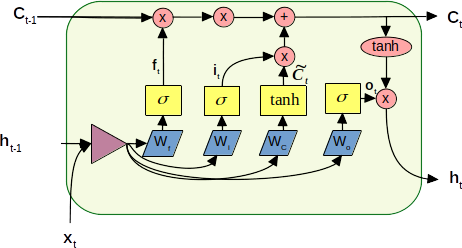
\includegraphics[width=0.6\textwidth]{Fig1.png}
\caption{LSTM neuron structure}\label{fig1}
\end{figure}

Where:
\begin{itemize}
\item $C_{t-1},C_t$ are the context vectors from the  previous and current time steps respectively.
\item $h_{t-1}, h_t$ are the output vectors from the previous and current time steps respectively.
\item $f_t$ is the vector produced by the forget gate.
\item $i_t$ is the vector produced by the input activate gate at the current time step.
\item $\tilde{C_t}$ is the vector produced by the input modulation gate at the current time step.
\item $o_t$ is the vector produced by the output gate at the current time step.
\end{itemize}

Mathematically, LSTM neuron can be represented as follows:

\begin{align}
f_t &= \sigma( W_f \cdot [h_{t-1},x_t] + b_f) \nonumber \\
i_t &= \sigma( W_i \cdot [h_{t-1},x_t] + b_i) \nonumber \\
\tilde{C_t} &= tanh( W_C \cdot [h_{t-1},x_t] + b_C) \nonumber \\
C_t &= f_t * C_{t-1} + i_t * \tilde{C_t} \nonumber \\
o_t &= \sigma( W_o \cdot [h_{t-1},x_t] + b_o) \nonumber \\
h_t &= o_t * tanh(c_t) \label{eq6}
\end{align}

A GRU neuron is essentially a simplified version of the LSTM neuron with its scheme presented on Figure \ref{fig2}:
\begin{figure}[H]
\centering
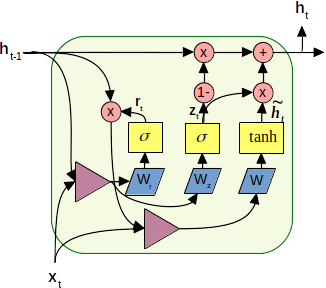
\includegraphics[width=0.45\textwidth]{Fig2.png}
\caption{GRU neuron structure}\label{fig2}
\end{figure}

In this neuron, the output vector $h_t$ also performs the role of the context vector, and the following blocks are used:

\begin{itemize}
\item Update block $z_t(x_t,h_{t-1};W_z)$ that calculates weights in the range $(0, 1)$, which are used to calculate a new output vector (and, at the same time, context) $h_t$ based on the candidate vector $\tilde{h}_t$ and the previous vector $h_{t-1}$
\item Relevance block $r_t(x_t,h_{t-1};W_r)$ that calculates weights in the range $(0, 1)$ which determine the relevance of the values of the previous output vector $h_{t-1}$ when calculating the candidate vector for the new output vector $\tilde{h}_t$
\item Block for calculating the candidate vector of new outputs $\tilde{h}_t(x_t,h_{t-1},r_t;W)$
\item A block for calculating a new output vector $h_t(h_{t-1},\tilde{h}_t,z_t)$  as a weighted sum of the corresponding values from the previous vector $h_{t-1}$ and a new candidate vector $\tilde{h}_t$, where the weights for the values under index $i$ are chosen as $1-z_t[i]$ and $z_t[i]$ respectively. 
\end{itemize}

\section{Recurrent Sigmoid Piecewise Linear Neuron}\label{sec5}
\subsection{Sigmoid Piecewise Linear neuron and its features}\label{subsec51}
Any continuous function $f: \mathbb{R}^n \to \mathbb{R} $ can always be approximated via a piecewise linear function that divides the space $\mathbb{R}^n$ into non-overlapping convex regions $S_1,S_2,...,S_N \in \mathbb{R}^n, S_i \cap S_j = \emptyset $  and defines a separate linear function $f_i(x) = w_i \cdot x, w_i \in \mathbb{R}^n.$ for each region. Consider a simple piecewise linear neuron as a basic element for generating such complex piecewise linear functions:
\begin{equation}
  pl(x;w_+,w_-,h) =
    \begin{cases}
      w_+ \cdot x & \text{if $h \cdot x \ge 0$}\\
      w_- \cdot x & \text{if $h \cdot x < 0$}
    \end{cases}
    , w_+, w_-, h \in \mathbb{R}^n \label{eq7}
\end{equation}
Parameters vectors $w_+,w_-,h$ have the following meaning: 
\begin{itemize}
\item $h \in \mathbb{R}^n$ defines a hyperplane that splits $\mathbb{R}^n$ in 2 halves
\item $w_+$ defines a linear function for the region where $h \cdot x \ge 0$
\item $w_-$ defines a linear function for the region where $h \cdot x < 0 $
\end{itemize}
The function $pl$ is obviously non-differentiable and not continuous at $x$ s.t. $h \cdot x = 0$. This issue can be resolved by using the following neuron model, called sigmoid piecewise linear (SPL) neuron:
\begin{equation}
spl(x;w_+,w_-,h) = \frac{w_+ \cdot x}{1 + e^{-h \cdot x}} + \frac{w_- \cdot x}{1 + e^{h \cdot x}}. \label{eq8}
\end{equation}
If we rewrite piecewise linear neuron as:
\begin{equation}
pl(x;w_+,w_-,h) = (w_+ \cdot x) \cdot \boldsymbol{1}_{[0;\infty)}(h \cdot x) + 
   (w_- \cdot x) \cdot \boldsymbol{1}_{(-\infty;0)}(h \cdot x) \label{eq9}
\end{equation}
we see that SPL neuron essentially replaces step functions $\boldsymbol{1}_{[0;\infty)}(h \cdot x)$ and $\boldsymbol{1}_{(-\infty;0)}(h \cdot x)$ with sigmoid functions $ \sigma_+(x;h) = \frac{1}{1 + e^{-h \cdot x}} $ and $ \sigma_-(x;h) = \frac{1}{1 + e^{h \cdot x}} $ respectively, and sigmoid function can be viewed as a smooth approximation of the step function, with both functions graphs presented on Figure \ref{fig3}:

\begin{figure}[H]
\centering
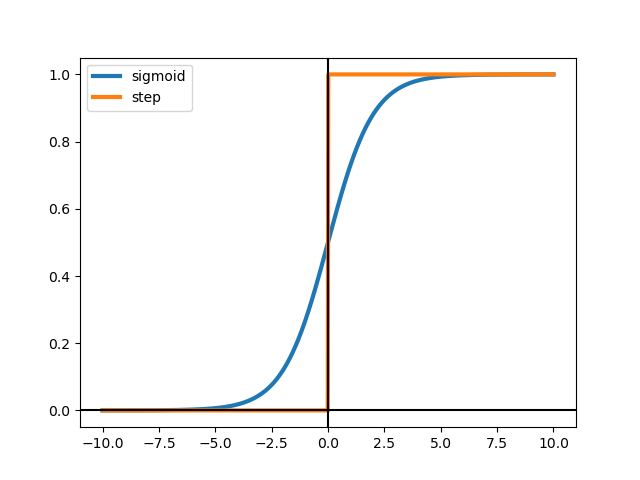
\includegraphics[width=0.7\textwidth]{Fig3.png}
\caption{Comparison of step and sigmoid functions}\label{fig3}
\end{figure}

Standard artificial neuron consists of two parts: a weighted adder $s(x;w) = w \cdot x$ and an activation function $a(y; \theta)$ (where $\theta$ is an optional vector of activation function's parameters), and the neuron itself is a composition of these parts:
\begin{equation}
f(x;w,\theta)=a(s(x;w);\theta)=a(w \cdot x; \theta) \label{eq10}
\end{equation}
In the case of SPL neuron the structure is somewhat more complicated: it consists of 3 weighted adders blocks $s_+(x;w_+),s_-(x;w_-),s_h(x;w_h)$ and an activation function of 3 variables:
\begin{equation}
a(s_+,s_-,s_h) = \frac{s_+}{1 + e^{-s_h}} + \frac{s_-}{1 + e^{s_h}}, \label{eq11}
\end{equation}
that together compose "into" SPL neuron:
\begin{equation}
 spl(x;w_+,w_-,w_h) = a(s_+(x;w_+),s_-(x;w_-),s_h(x;w_h)). \label{eq12}
 \end{equation}
 Unfortunately, because the SPL neuron's activation function is a function of three variables it is not  possible to plot it as a two- or three-dimensional graph. However, we can plot the graph with some additional constraints. For example, the three dimensional plot of the activation function with an added constraint $S_+=5S_-$ is presented on Figure \ref{fig4}:

\begin{figure}[H]
\centering
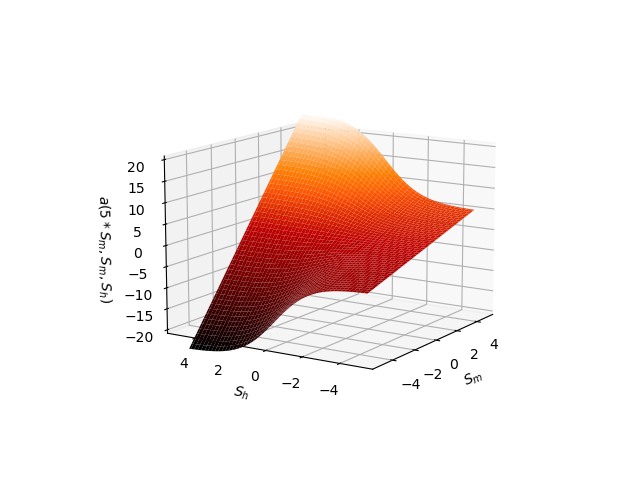
\includegraphics[width=0.7\textwidth]{Fig4.png}
\caption{3D plot of SPL neuron's activation function with added constraint $S_p=5S_m$}\label{fig4}
\end{figure}

In the context of building a predictive model for non-stationary time series with several potential conditional distributions, the Sigmoid Piecewise neuron can be considered as one of the simplest predictive models consisting of several local models and a component model that determines which of the local models to apply to a given input vector. That is, parameter vector $w_+$ specifies the first local model corresponding to one of the two potential distributions, vector $w_-$ – the second local model corresponding to the second potential distribution, and vector $h$ – the parameters of the component model that, according to the values of the input vector, determines which potential distribution is active - and therefore which local model to use to get the forecast. By combining several such neurons, it is already possible to simulate more than two potential conditional distributions. 
 
\subsection{Training the parameters of SPL neuron}\label{subsec52}
Since the mathematical model of the Sigmoid Piecewise neuron is a differentiable function of its parameters, their adjustment to minimize a certain function that depends on the output of the neuron can be performed using a certain modification of the gradient descent algorithm, using the following formulas for calculating the first derivatives:
\begin{align}
\frac{\partial f}{\partial w_{+(q)}} &= \frac{x_q}{1+e^{-h \cdot x}}, \label{eq13} \\
\frac{\partial f}{\partial w_{-(q)}} &= \frac{x_q}{1+e^{h \cdot x}}, \label{eq14} \\
\frac{\partial f}{\partial h_q} &=-\frac{w_+ \cdot x}{(1+e^{-h \cdot x})^2}e^{-h \cdot x}(-x_q)
	-\frac{w_- \cdot x}{(1+e^{h \cdot x})^2}e^{h \cdot x}x_q= \nonumber \\
 &= \frac{(w_+ \cdot x)x_q}{(1+e^{-h \cdot x})(1+e^{-h \cdot x})e^{h \cdot x}}-
	\frac{(w_- \cdot x)x_q}{(1+e^{h \cdot x})(1+e^{h \cdot x})e^{-h \cdot x}}=  \nonumber \\
 &=\frac{(w_+ \cdot x)x_q}{(1+e^{-h \cdot x})(1+e^{h \cdot x})}-
	\frac{(w_- \cdot x)x_q}{(1+e^{h \cdot x})(1+e^{-h \cdot x})}=  \nonumber \\
 &=\frac{(w_+ \cdot x)x_q - (w_- \cdot x)x_q}{(1+e^{-h \cdot x})(1+e^{h \cdot x})}=  \nonumber \\
& =\frac{x_q(w_+ \cdot x - w_- \cdot x)}{2+e^{-h \cdot x} + e^{h \cdot x}} \label{eq15}
\end{align}
3D plots for the derivatives $\frac{\partial f}{\partial w_{+(q)}}$ and $\frac{\partial f}{\partial w_{-(q)}}$ as functions of variables $x_q$ and $s_h=h \cdot x$ are presented on Figure \ref{fig5}:

\begin{figure}[H]
\centering
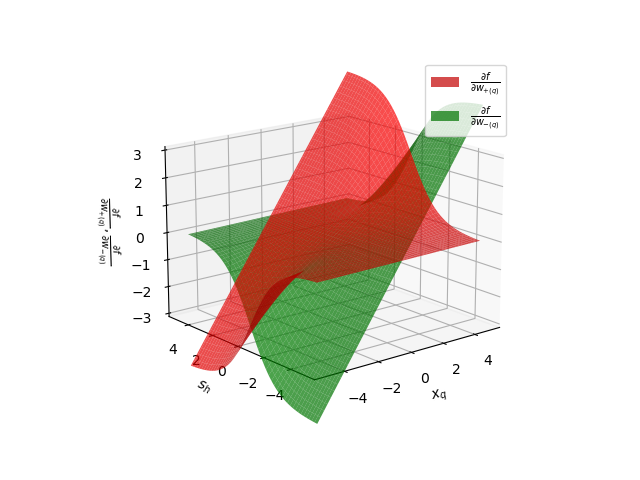
\includegraphics[width=0.7\textwidth]{Fig5.png}
\caption{3D plots of SPL neuron's partial derivatives w.r.t. $w_{+(q)}$ and $w_{-(q)}$}\label{fig5}
\end{figure}

And the plot of the derivative $\frac{\partial f}{\partial h_q}$ as function of the variables $t=x_q(w_+ \cdot x - w_- \cdot x)$ and $s_h=h \cdot x$ is shown on Figure \ref{fig6}:

\begin{figure}[H]
\centering
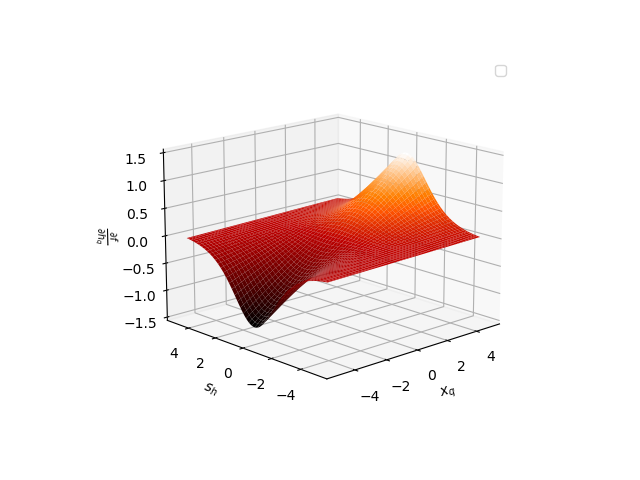
\includegraphics[width=0.7\textwidth]{Fig6.png}
\caption{3D plot of SPL neuron's partial derivative w.r.t. $h_q$}\label{fig6}
\end{figure}

For further analysis of the "behavior" of the partial derivatives of the SPL neuron, it is also worth noting that the sum $\frac{\partial f}{\partial w_{+(q)}} + \frac{\partial f}{\partial w_{-(q)}}$ can be simplified as follows:
\begin{align}
\frac{\partial f}{\partial w_{+(q)}} + \frac{\partial f}{\partial w_{-(q)}} &= 
	\frac{x_q}{1+e^{-h \cdot x}} + \frac{x_q}{1+e^{h \cdot x}} = \nonumber \\
\frac{x_q (1+e^{h \cdot x}) + x_q(1+e^{-h \cdot x})}{(1+e^{-h \cdot x})(1+e^{h \cdot x)}} &=
	\frac{x_q (2+e^{h \cdot x}+e^{-h \cdot x})}{2+e^{h \cdot x}+e^{-h \cdot x}} = x_q \label{eq16}
\end{align}
After analyzing these graphs and equations, the following conclusions can be drawn: 
\begin{enumerate}
\item The value $S_h=h \cdot x$ has an important influence on the value of all derivatives, that is, how far and on which side from the dividing plane specified by the vector $h$ is the input vector $x$.
\item Equation \ref{eq16} shows that sum of derivatives $\frac{\partial f}{\partial w_{+(q)}} + \frac{\partial f}{\partial w_{-(q)}}$ is always equal to $x_q$. However, depending on the sign and the magnitude of $S_h$ the contribution of $\frac{\partial f}{\partial w_{+(q)}}$ and $\frac{\partial f}{\partial w_{-(q)}}$ will be different: if $S_h << 0$ - the value of $\frac{\partial f}{\partial w_{+(q)}}$ will be close to 0 and the value of $\frac{\partial f}{\partial w_{-(q)}}$ will be close to $x_q$, and vice versa when $S_h >> 0$. When $S_h \approx 0$ - contribution of both derivatives will be similar.
\item From Equation \ref{eq15} we see that the derivative $\frac{\partial f}{\partial h_q} \approx 0 $ when $|S_h| >> 0 $ and $\approx \frac{x_q(w_+ \cdot x - w_- \cdot x)}{4}$ when $S_h \approx 0$. Thus, if the vector $x$ is far from the separating hyperplane defined by $h$ - it won't influence the training of vector $h$ very much. On the other hand, if $x$ is close to the hyperplane (i.e. $S_h \approx 0$) - the derivative $\frac{\partial f}{\partial h_q} $ will be proportional to $(w_+ \cdot x - w_- \cdot x)$. So the biggest influence on the correction of $h$ will be "caused" by inputs vectors $x$ such that: $h \cdot x \approx 0$ and $|w_+ \cdot x - w_- \cdot x| >> 0$. Besides that, if at some point during training all input vectors $x$ will have $h \cdot x >> 0$ - correction of $h$ will practically stop, since all derivatives $\frac{\partial f}{\partial h_q}$ will be close to 0. This can happen in two cases:
\begin{enumerate}
\item All input vectors are on 1 side of the separating hyperplane defined by $h$ - in this case SPL neuron will essentially be equivalent to the ordinary linear neuron, and only one of the vectors $w_+$ or $w_-$ will be tuned.
\item Some input vectors are on 1 side of the hyperplane and some are on another side, i.e. there are 2 clusters in input vectors which are linearly separable with a certain gap and we've found a corresponding "separation" hyperplane. In most practical cases this can be considered a good outcome, since we would probably want different linear models applied to different clusters of data. 
\end{enumerate}
\item If after some training step the vectors $w_+$ and $w_-$ become close - the derivative $\frac{\partial f}{\partial h_q}$ will be close to 0. However taking into account previous analysis items we can conclude that this situation will not last too long unless all input vectors lie on the separating hyperplane defined by $h$.
\end{enumerate}
  
 To use the SPL neuron in multilayer neural networks, in addition to the derivative of the neuron function w.r.t. its parameters the derivative w.r.t. to the input variables $x_q$ is also required:
 \begin{align}
\frac{\partial f}{\partial x_q} &= \frac{h_q(w_+ \cdot x - w_- \cdot x)}
	{2+e^{-h \cdot x} + e^{h \cdot x}} + \frac{w_{+(q)}}{1 + e^{-h \cdot x}} +
	\frac{w_{-(q)}}{1 + e^{h \cdot x}} = \nonumber \\
&= \frac{\partial f}{\partial h_q}\frac{h_q}{x_q} + \frac{w_{+(q)}}{1 + e^{-h \cdot x}}
	+ \frac{w_{-(q)}}{1 + e^{h \cdot x}} \label{eq17}
\end{align} 
 
 From this equation we can conclude that $\frac{\partial f}{\partial x_q}$ will be non-zero whenever $w_{+(q)} \ne 0 $ or $w_{_(q)} \ne 0$. 

\subsection{Recurrent SPL neuron and its features}\label{subsec53}
We propose a new recurrent neuron called Recurrent Sigmoid Piecewise Linear neuron (RSPL) which is based on the SPL neuron. So, we start at standard single SPL neuron:
\begin{equation}
SP(x;w_+,w_-,s) = (1 - \sigma(x;s))(w_- \cdot x) + \sigma(x;s)(w_+ \cdot x) \label{eq18}
\end{equation}
Now, if we need to describe a layer of SPL neurons then vectors $w_+,w_-,s$ will be replaced by the matrices  $W_+,W_-,S$:
\begin{equation}
SP(x;W_+,W_-, S) = (1 - \sigma(x;S)) * (W_- \cdot x) + \sigma(x;S) * (W_+ \cdot x) \label{eq19}
\end{equation}
By introducing the notation $ z = \sigma(x;S) $, $a = W_- \cdot x$  and $b = W_+ \cdot x$ we obtain:
\begin{equation}
SP(x) = (1 - z) * a + z * b \label{eq20}
\end{equation}
Which is similar to the block for calculating the new context vector in the GRU/LSTM neuron (as in Equation \ref{eq6}). Thus, by slightly changing the SPL neuron, you can get its recurrent version, the RSPL neuron, which takes the vector $p_t=[h_{t-1}, x_t]$ as input and produces vector $h_t$ that serves both as context and as output vector:
\begin{equation}
h_t=RSP(p_t;W_c,S) = (1-\sigma(p_t;S))*p_t + \sigma(p_t;S)*(W_c \cdot p_t) \label{eq21}
\end{equation}
Or, by analogy with LSTM/GRU neurons, the mathematical model of an RSPL neuron can be written in several stages/blocks:
\begin{align}
z_t &= \sigma(S \cdot [h_{t-1}, x_t]) \nonumber \\
\tilde{h}_t &= W_c \cdot [h_{t-1}, x_t] \nonumber \\
h_t &= (1 - z_t) * h_{t-1} + z_t * \tilde{h}_t \label{eq22}
\end{align}
And present them in the form of the scheme shown on Figure \ref{fig7}:

\begin{figure}[H]
\centering
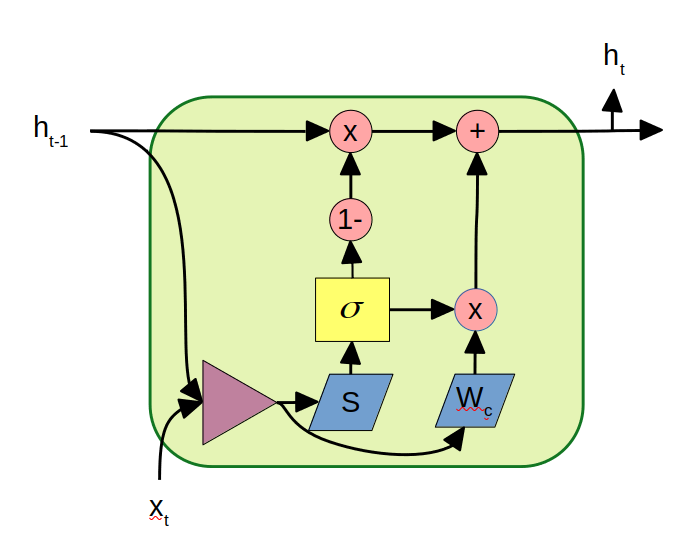
\includegraphics[width=0.5\textwidth]{Fig7.png}
\caption{RSPL neuron structure}\label{fig7}
\end{figure}

By performing a simple comparison of the RSPL neuron with LSTM and GRU neurons following observations can be made:

\begin{itemize}
\item The mathematical model of the RSPL neuron is simpler (only one nonlinear sigmoidal block is used) than the models of LSTM and GRU neurons. In the problem of time series forecasting, simpler models are often preferred in practice. 
\item At the same time, RSPL, as well as LSTM and GRU neurons, allows you to forget certain values in the context vector if necessary. 
\end{itemize}

\section{RSPL neuron evaluation}\label{sec6}
To evaluate the effectiveness of using the RSPL neuron in modeling the predicted time series, two real time series were used: 

\begin{itemize}
\item Daily values of the Dow Jones index for the period 2015/01/01-2023/1/1, total length of the time series - 2014 values, with the series' plot as shown on Figure \ref{fig8}:
\begin{figure}[H]
\centering
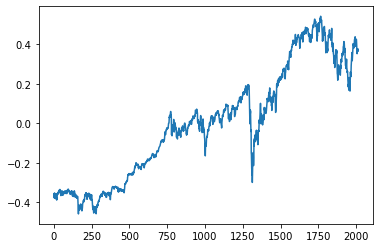
\includegraphics[width=0.5\textwidth]{Fig8.png}
\caption{Dow Jones index daily values time series plot}\label{fig8}
\end{figure}
\item OT (oil temperature) time series from the Electricity Transformer Dataset, which is often used to evaluate forecasting methods, with a total time series length of 5000 values \citep{haoyietal-informer-2021}, with the plot shown on Figure \ref{fig9}:
\begin{figure}[H]
\centering
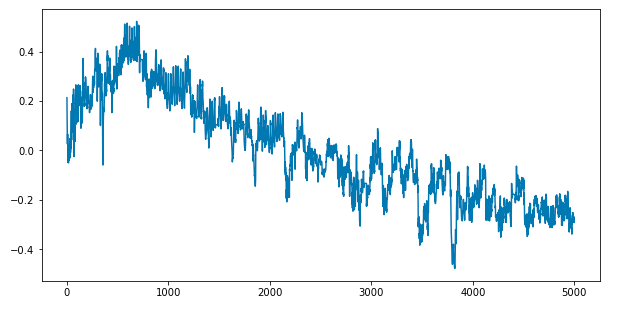
\includegraphics[width=0.5\textwidth]{Fig9.png}
\caption{Plot of oil temperature time series from the Electricity Transformer dataset}\label{fig9}
\end{figure}
\end{itemize}

These series were divided into training and test sets, after which the model parameters were adjusted on the training set and metrics were calculated on the test set. To bring the original time series to a “more stationary form,” an optimal linear predictor was first selected for each training sample, after which the corresponding recurrent network was “set” with the task of predicting the deviation of the real value of the time series from the forecast of the linear predictor. Two previous values of the time series were used as input to the network to predict the next value; the learning rate for all models was set to 0.001, maximum number of training epochs to 300. To compare RSPL neuron with LSTM and GRU in various network configurations, the following values of hyperparameters were tested: number of network layers $\in [1, 3, 5]$, dimension of the hidden state vector $\in [4, 8, 32]$.
In total, given 3 choices for the neuron type, 3 choices for the number of layers, and 3 choices for the dimension of the hidden state vector, 27 different models were trained for each time series. For each model, the error values on the test set were calculated once every 20 training epochs, and the time spent on completing each epoch was also logged. Summary of the obtained results is presented in Table \ref{table1} and Table \ref{table2}:
\\
\begin{table}[H]
\caption{Results summary for different network configurations on the Dow Jones index time series}\label{table1}
\begin{tabular}{|p{1.4cm}|p{1.4cm}|p{1.4cm}|p{1.5cm}|p{2.5cm}|p{1.9cm}|p{2cm}|}
\hline
Number of layers & Hidden layer size & Neuron type & Best test error & Relative best test error & Mean epoch time (s) & Relative mean epoch time\\
\hline
 1 &   4 &   RSPL & 0.0065 & 1.0427 & 0.5714 &  1.0000 \\
\hline
 1 &   4 &   GRU & 0.0080 & 1.2818 & 0.6393 &  1.1187 \\
\hline
 1 &   4 &  LSTM & 0.0062 & 1.0000 & 0.7121 &  1.2461 \\
\hline
 1 &   8 &   RSPL & 0.0063 & 1.0236 & 0.5749 &  1.0000 \\
\hline
 1 &   8 &   GRU & 0.0063 & 1.0176 & 0.6477 &  1.1266 \\
\hline
 1 &   8 &  LSTM & 0.0062 & 1.0000 & 0.7148 &  1.2434 \\
\hline
 1 &  32 &   RSPL & 0.0062 & 1.0000 & 0.5790 &  1.0000 \\
\hline
 1 &  32 &   GRU & 0.0062 & 1.0001 & 0.6602 &  1.1404 \\
\hline
 1 &  32 &  LSTM & 0.0063 & 1.0128 & 0.7805 &  1.3482 \\
\hline
 3 &   4 &   RSPL & 0.0068 & 1.0794 & 1.3176 &  1.0000 \\
\hline
 3 &   4 &   GRU & 0.0063 & 1.0000 & 1.5118 &  1.1475 \\
\hline
 3 &   4 &  LSTM & 0.0067 & 1.0753 & 1.8286 &  1.3879 \\
\hline
 3 &   8 &   RSPL & 0.0067 & 1.0796 & 1.3112 &  1.0000 \\
\hline
 3 &   8 &   GRU & 0.0063 & 1.0292 & 1.5177 &  1.1575 \\
\hline
 3 &   8 &  LSTM & 0.0062 & 1.0000 & 1.8187 &  1.3870 \\
\hline
 3 &  32 &   RSPL & 0.0062 & 1.0097 & 1.3277 &  1.0000 \\
\hline
 3 &  32 &   GRU & 0.0062 & 1.0041 & 1.5323 &  1.1541 \\
\hline
 3 &  32 &  LSTM & 0.0061 & 1.0000 & 1.9881 &  1.4975 \\
\hline
 5 &   4 &   RSPL & 0.0063 & 1.0179 & 2.0749 &  1.0000 \\
\hline
 5 &   4 &   GRU & 0.0069 & 1.0998 & 2.4140 &  1.1635 \\
\hline
 5 &   4 &  LSTM & 0.0062 & 1.0000 & 2.9418 &  1.4178 \\
\hline
 5 &   8 &   RSPL & 0.0065 & 1.0263 & 2.0498 &  1.0000 \\
\hline
 5 &   8 &   GRU & 0.0063 & 1.0000 & 2.4031 &  1.1724 \\
\hline
 5 &   8 &  LSTM & 0.0071 & 1.1170 & 2.9154 &  1.4223 \\
\hline
 5 &  32 &   RSPL & 0.0065 & 1.0409 & 2.0939 &  1.0000 \\
\hline
 5 &  32 &   GRU & 0.0062 & 1.0067 & 2.4391 &  1.1649 \\
\hline
 5 &  32 &  LSTM & 0.0062 & 1.0000 & 3.1976 &  1.5271 \\
\hline
\end{tabular}
\end{table}

\begin{table}[H]
\caption{Results summary for different network configurations on the OT ETTH time series}\label{table2}
\begin{tabular}{|p{1.4cm}|p{1.4cm}|p{1.4cm}|p{1.5cm}|p{2.5cm}|p{1.9cm}|p{2cm}|}
\hline
Number of layers & Hidden layer size & Neuron type & Best test error & Relative best test error & Mean epoch time (s) & Relative mean epoch time \\
\hline
1 &   4 &   RSPL & 0.0030 & 1.0030 & 1.4462 &  1.0000 \\
\hline
1 &   4 &   GRU & 0.0030 & 1.0000 & 1.6299 &  1.1270 \\
\hline
1 &   4 &  LSTM & 0.0031 & 1.0334 & 1.8409 &  1.2729 \\
\hline
1 &   8 &   RSPL & 0.0030 & 1.0000 & 1.4436 &  1.0000 \\
\hline
1 &   8 &   GRU & 0.0030 & 1.0240 & 1.6246 &  1.1254 \\
\hline
1 &   8 &  LSTM & 0.0030 & 1.0021 & 1.8294 &  1.2672 \\
\hline
1 &  32 &   RSPL & 0.0029 & 1.0000 & 1.4709 &  1.0000 \\
\hline
1 &  32 &   GRU & 0.0030 & 1.0072 & 1.6553 &  1.1254 \\
\hline
1 &  32 &  LSTM & 0.0030 & 1.0164 & 1.9888 &  1.3521 \\
\hline
3 &   4 &   RSPL & 0.0031 & 1.0129 & 3.3214 &  1.0000 \\
\hline
3 &   4 &   GRU & 0.0031 & 1.0000 & 3.9134 &  1.1782 \\
\hline
3 &   4 &  LSTM & 0.0032 & 1.0281 & 4.6709 &  1.4063 \\
\hline
3 &   8 &   RSPL & 0.0031 & 1.0181 & 3.2960 &  1.0000 \\
\hline
3 &   8 &   GRU & 0.0030 & 1.0014 & 3.9221 &  1.1899 \\
\hline
3 &   8 &  LSTM & 0.0030 & 1.0000 & 4.6470 &  1.4099 \\
\hline
3 &  32 &   RSPL & 0.0030 & 1.0225 & 3.3440 &  1.0000 \\
\hline
3 &  32 &   GRU & 0.0029 & 1.0000 & 3.9690 &  1.1869 \\
\hline
3 &  32 &  LSTM & 0.0030 & 1.0269 & 5.0812 &  1.5195 \\
\hline
5 &   4 &   RSPL & 0.0030 & 1.0000 & 5.2663 &  1.0000 \\
\hline
5 &   4 &   GRU & 0.0031 & 1.0200 & 6.1705 &  1.1717 \\
\hline
5 &   4 &  LSTM & 0.0032 & 1.0841 & 7.6743 &  1.4573 \\
\hline
5 &   8 &   RSPL & 0.0030 & 1.0000 & 5.2238 &  1.0000 \\
\hline
5 &   8 &   GRU & 0.0031 & 1.0413 & 6.1681 &  1.1808 \\
\hline
5 &   8 &  LSTM & 0.0031 & 1.0230 & 7.6274 &  1.4601 \\
\hline
5 &  32 &   RSPL & 0.0030 & 1.0098 & 5.3234 &  1.0000 \\
\hline
5 &  32 &   GRU & 0.0030 & 1.0198 & 6.2275 &  1.1698 \\
\hline
5 &  32 &  LSTM & 0.0029 & 1.0000 & 8.3525 &  1.5690 \\
\hline
\end{tabular}
\end{table}

In these tables, "relative best test error" and "relative mean epoch time" were calculated by dividing the corresponding absolute value by the minimum value among all 3 neuron types for the given hyperparameters configuration. That is, for each specific configuration of the number of layers and the hidden layer size there are 3 rows, one for each type of neuron; among these 3 rows, the row for the neuron with the smallest absolute best test error will have a relative best test error value equal to 1, and all others will have some values >= 1, similarly for the absolute and relative mean epoch time. 

Aggregated results for Dow Jones index time series are presented in Table \ref{table3}, for ET OTTH time series - in Table \ref{table4} and results, aggregated over both time series are presented in Table \ref{table5}:

\begin{table}[H]
\caption{Aggregated results on the Dow Jones index time series}\label{table3}
\begin{tabular}{ |p{2.2cm}|p{5cm}|p{5cm}| }
 \hline
  Neuron type & Aggregated relative best test error & Aggregated relative mean epoch time \\
  \hline
 RSPL & 1.03556 & 1.0 \\
 \hline  
 GRU & 1.0488 & 1.1495 \\
 \hline 
 LSTM & 1.0228 & 1.38636 \\
 \hline
\end{tabular}
\end{table}

\begin{table}[H]
\caption{Aggregated results on the ET OTTH time series}\label{table4}
\begin{tabular}{ |p{2.2cm}|p{5cm}|p{5cm}|  }
 \hline
  Neuron type & Aggregated relative best test error & Aggregated relative mean epoch time \\
  \hline
 RSPL & 1.00736 & 1.0 \\
 \hline  
 GRU & 1.01264 & 1.16169 \\
 \hline 
 LSTM & 1.02377 & 1.4127 \\
 \hline
\end{tabular}
\end{table}

\begin{table}[H]
\caption{Aggregated results for both time series}\label{table5}
\begin{tabular}{ |p{2.2cm}|p{5cm}|p{5cm}|  }
 \hline
  Neuron type & Aggregated relative best test error & Aggregated relative mean epoch time \\
  \hline
 RSPL & 1.02146 & 1.0 \\
 \hline  
 GRU & 1.030724 & 1.1556 \\
 \hline 
 LSTM & 1.02328 & 1.3995 \\
 \hline
\end{tabular}
\end{table}

Overall summary regarding RSPL neuron: 

• for the DJI series, the relative best test error averaged over all configurations ranks 2nd after LSTM 

• for the OT ETTH series - 1 place 

• relative time per epoch, averaged over all configurations for both series is 1.0, which is approximately 15.5\% faster than the next “fastest” neuron – GRU 

• If we average the relative best test error over all configurations and over both time series, RSPL takes 1st place. 

To compare pure inference speed of the RSPL neuron we measure the average computation time of networks with GRU and RSPL neurons among 100,000 runs for different values of the input vector size and hidden layer size. The LSTM neuron, as is known from the literature, is generally slower than the GRU. Results of performed computation time measurements are presented in Table \ref{table6}:

\begin{table}[H]
\caption{Average computation time of networks with GRU/RSPL neurons and different configurations}\label{table6}
\begin{tabular}{ |p{2cm}|p{2cm}|p{2cm}|p{2cm}|p{2cm}|p{2cm}|  }
 \hline
  Input and hidden layer size & 8, 64 & 4, 12 &  4, 32 & 2, 8 & 2, 16 \\
  \hline
 GRU & 0.054 ms & 0.0487 ms & 0.0503 ms & 0.0492 ms & 0.0507 ms \\
 \hline 
 RSPL & 0.0355 ms & 0.032 ms & 0.0327 ms & 0.0317 ms & 0.032 ms \\
 \hline
\end{tabular}
\end{table}

As can be seen from the Table \ref{table6}, networks with RSPL neuron are on average 1.58 times faster than networks of the same structure with GRU neuron.

\section{Conclusion}\label{sec7}
In this paper, we have presented a new recurrent neuron - RSPL, that could be used in neural networks for modeling time series forecasting. It is based on the sigmoid piecewise linear neuron and can be viewed as a simplified version of a well known GRU recurrent neuron. RSPL neuron could be used as a drop-in replacement in any networks that use LSTM or GRU neurons.

Real-world data analyses on multiple time series and multiple neural network configurations have shown that networks with RSPL neurons achieve similar or better accuracy on the test set when compared with networks that use LSTM or GRU neurons. At the same time, training and inference speed for networks with RSPL neurons is noticeably faster.

\bibliography{paper}

\end{document}


